\documentclass[a4paper,10pt]{article}
\usepackage[british]{babel}
\usepackage[T1]{fontenc}
\usepackage[hidelinks]{hyperref}
\usepackage[a4paper]{geometry}

\usepackage{tabularx}
\usepackage{graphicx}
\usepackage{rotating}
\usepackage{float}
\usepackage{xspace}

% Math packages
\usepackage[sc]{mathpazo}
\usepackage{amsthm}
\usepackage{algorithmic}
\usepackage{amsmath}

\usepackage{listings}

% Document properties
\title{Welch-Lynch clock synchronization protocol \\\textit{Modelling in UPPAAL}}
\author{
	Wouter Geraedts \\ \small{\texttt{w.geraedts@student.ru.nl}} \and
	Ko Stoffelen     \\ \small{\texttt{kostoffelen@student.ru.nl}}
}
\date{}
\linespread{1.05}

% Terminology
\newcommand{\UPPAAL}{UPPAAL\xspace}

\begin{document}
	\maketitle

%%% Contents %%%
%Originele paper

%Zoeken naar concrete constanten

%Aanpassingen voor snelheid
%	Gebruik van C-functies [step1]
%	Gebruik van select-statements [step2]
%	Gebruik van local_time uit originele paper [step3]
%	Gebruik van SUM uit originele paper [step3minimized]
%	Timejumps [step3minimized]
%	Scalarset reduction [step4scalar]
%	Uitgebreide guards (forall i.p.v. local var C) [step2]

%Aanpassingen voor generiekerheid
%	Diff variable upgrade
%	Concrete types
%	Min en max (zelfs trager dan SUM) [step4]

%Resultaten: Vergelijkingen in performance
%Faulty process, niet mogelijk
%	Werk om te doen om het alsnog te maken (array voor min en max; zorgen dat het kan met scalarset (id_t))

\section{Introduction}

%Over dit paper
%Relatie met originele paper
%Opbouw van dit paper
%Korte verwijzing naar conclusie

This report is part of an assignment for the Analysis of Embedded Systems course in 2012--2013. Our goal was to model and analyze the Welch-Lynch fault-tolerant clock synchronization protocol \cite{Welch1984Anew} using \UPPAAL. A previous attempt has been made in 2004 \cite{Aceto2004Notes}, when the model had to be greatly simplified. New \UPPAAL features like symmetry reduction, a richer syntax and a more powerful verification engine in general, make that the model-based analysis deserved another chance.

The algorithm in its most general form still does not directly translate to an \UPPAAL model that is actually verifiable. This report first describes what optimizations, simplifications and updates have been applied to a general model. Then in section~\ref{sec:faulty} it is explained what else would have been needed to be able to verify a general version of the protocol. In section~\ref{sec:remarks} some remarks are made on \cite{Aceto2004Notes}, which explain some troubles that appeared in the process of this analysis. Finally in section~\ref{sec:performance} the performance of our optimized model is compared to the 2004 version, after which we draw our conclusions. \UPPAAL is able to verify the correctness of the protocol for three participating processes with a highly optimized model, but then we are already approaching the limit of \UPPAAL{}s capabilities.

\section{Optimizations}

In 2004, a model was made that models the protocol in almost its most general form. However, fault-tolerance is completely ignored and a trick is applied to model the floating point numbers that correspond to clocks. This has been our starting point of reference. The most important automaton, the description of a process, can be seen in figure~\ref{fig:original_process}.

\begin{figure}[!h]
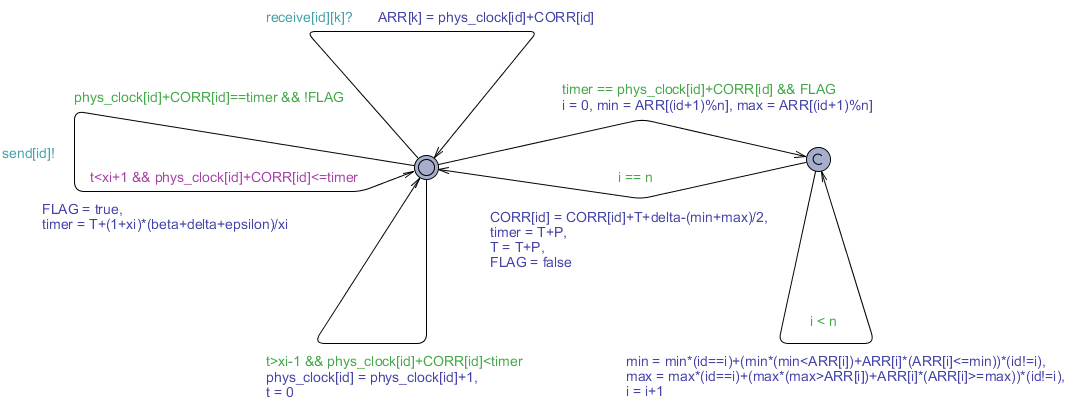
\includegraphics[width=\textwidth]{original_process}
\label{fig:original_process}
\end{figure}

It was soon getting clear that all other optimizations had to be applied as well and even additional ones. Below is a complete list of all optimization steps that have been used and how they contribute to making the model verifiable.

\begin{enumerate}
\item \textbf{C-like functions} \\
	The \UPPAAL C-like declaration language has been enriched extensively over the years. For instance, in 2004, one was not able to use functions and complicated constructions had to be thought off to simulate the behaviour. In figure~\ref{fig:original_process}, the right part uses a committed state to iterate over an array to determine its minimal and maximal values. A similar structure is seen in the channel automaton. Luckily the new syntax allows us to replace these structures by C-like functions. Due to the nature of a committed state, this does not directly highly decrease the state space, but it allows for the removal of some variables, transitions and complex update statements. This at least makes the model more comprehensible. The result can be seen in figure~\ref{fig:step1_process}.

\begin{figure}[!h]
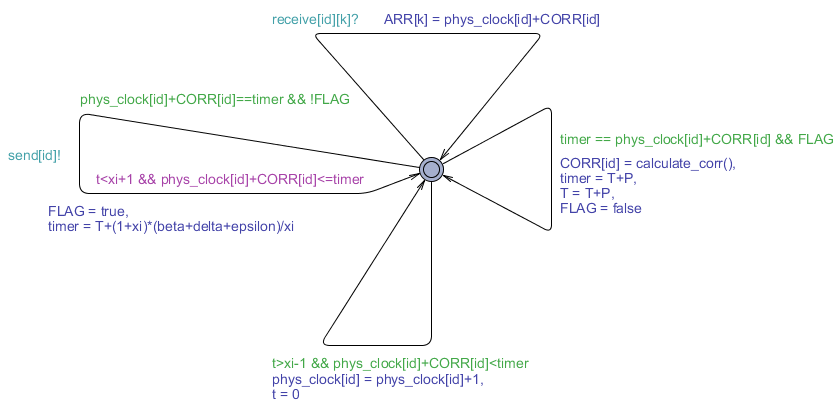
\includegraphics[width=\textwidth]{step1_process}
\label{fig:step1_process}
\end{figure}

\item \textbf{Select statements} \\
	The 2004 model uses two \textit{choice variable} automatons to let each process and each channel non-deterministically choose which message to receive. The automatons are used to iterate over all process instances. Such choice variables can now easily be replaced by select statements that range over some type \texttt{id\_t}. This reduces the state space. All iterating is now done implicitly within one single transition, without branching the search space.

\item \textbf{Rewriting variables} \\
	The \UPPAAL verification engine can not deal with unbounded integers very well. To solve this, it was proposed in 2004 to rewrite lots of variables in such a way that one can work with bounded variables. The main idea is to introduce the notion of a round explicitly in the description of a process. This is implemented by subtracting the round index multiplied with the time between rounds from all timer variables. Now effectively, these timers can only take values up to the time between rounds, a constant \(P\). Then some invariants are used to further reduce the number of variables. The correctness property is also altered by this, but it can be proven that the systems are equivalent.

\item \textbf{Specific three process instance} \\
	In 2004, it was probably noticed that it turned out to be hard to verify instances of the protocol using \UPPAAL. Therefore, the researchers tried to restrict themselves to three processes. This allows for a more direct computation of the minimum and maximum values in the right part of the process automaton. The variables \texttt{ARR1}, \texttt{min1} and \texttt{max1} are replaced by a single variable \texttt{SUM}. Removing variables implies reducing the search space.

\item \textbf{Time jumps} \\
	When traces were simulated within the model, it was noticed that for the larger part of the time, most variables were not changing values, except for the \texttt{local\_time} variable which was simply incrementing. When the counter reached 0, all process instances started to send out and receive messages. Before and after that, nothing changed within the system. This lead to the invention of a time jump optimization, where a process is allowed to simply skip the parts where nothing interesting is happening. Of course it has been made sure that the time jumps do not influence the total behaviour of the system in any way. This optimization has been shown to greatly reduce the state space. The resulting process automaton can be seen in figure~\ref{fig:step3minimized_process}.

\begin{figure}[!h]
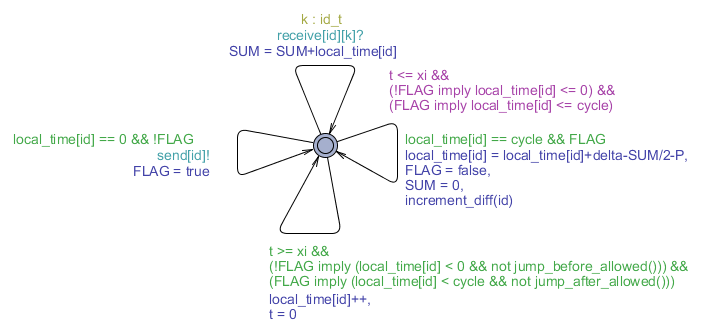
\includegraphics[width=\textwidth]{step3minimized_process}
\label{fig:step3minimized_process}
\end{figure}

\item \textbf{Symmetry reduction} \\
%TODO

\item \textbf{Extended guards} \\
%TODO
\end{enumerate}

%Aanpassingen voor snelheid
%Toelichten dat het leesbaarder is a.d.v. A First Introduction to UPPAAL

\section{Towards faulty process\label{sec:faulty}}

%Aanpassingen voor generiekerheid
%Aanpassingen die we nog wilde doen, indien we 5 processen hadden kunnen modelleren

\section{Remarks on \cite{Aceto2004Notes}\label{sec:remarks}}

%Niet duidelijk of ze daadwerkelijk het model hebben kunnen doorrekenen
%Geen concrete waarden voor constanten; beschrijving van zoektocht
%Onduidelijk wat het type is van variablen

\section{Performance\label{sec:performance}}

%Vergelijking tussen verschillende versies van ons, en uiteindelijke versie van aceto2004notes

\section{Conclusion}
	
%We kunnen succesvol 3 processen door laten rekenen, sneller dan toen (40 sec vs. <TODO>)
%Als 4 haalbaar blijkt te zijn, dan dat.
%5 nodig voor Faulty Process-eigenschap.

\bibliographystyle{plain}
\bibliography{main}

\end{document}
